\documentclass{article}

\usepackage{amsmath,amsfonts,amsthm,enumerate,bm}

%\VignetteIndexEntry{metaplus Example}
\usepackage[authoryear,round]{natbib}
\bibliographystyle{plainnat}

\title{metaplus Examples}
\author{Ken Beath\\Macquarie University\\ken.beath@mq.edu.au}

\usepackage{Sweave}
\begin{document}

\maketitle



In the following examples, both the robust options are used to demonstrate the capabilities of the package. In practice a choice will be made to use only one. The advantage of the mixture robust is that it gives the posterior probabilities that each study is an outlier. However it involves an extra parameter, so may be more unstable when fitting only a small number of studies.

\section{Intravenous Magnesium in Acute Myocardial Infarction}

A number of studies have been performed to determine the effectiveness of intravenous magnesium in acute myocardial infarction, and the data obtained from \cite{Sterne2001}. Of interest is, whether given the heterogeneity between studies, the ISIS-4 study is unusual.
We can perform the standard random effects meta-analysis, and parameter estimates as follows:
\begin{Schunk}
\begin{Sinput}
> data(mag)
> mag.meta <- metaplus(mag$yi,mag$sei,slab=mag$study)
> summary(mag.meta)
\end{Sinput}
\begin{Soutput}
         Est.   ci.lb   ci.ub   pvalue
muhat -0.7463 -1.2583 -0.3428 0.000501
tau2   0.2540                         

     logLik      AIC      BIC
  -19.68459 43.36918 44.91436
\end{Soutput}
\end{Schunk}

Adding \texttt{plotci=TRUE} will add a plot giving details of the profile confidence intervals, and is shown in Figure~\ref{fig:profile1}. When the quadratic approximation to the likelihood holds the shape of the curve will be in the form of a "V". In this case, the shape is not symmetric, so this does not hold. This is confirmed by the lack of symmetry of the confidence interval for muhat. 

\begin{figure}
  \centering
\begin{Schunk}
\begin{Sinput}
> mag.meta <- metaplus(mag$yi,mag$sei,slab=mag$study,plotci=TRUE)
\end{Sinput}
\end{Schunk}
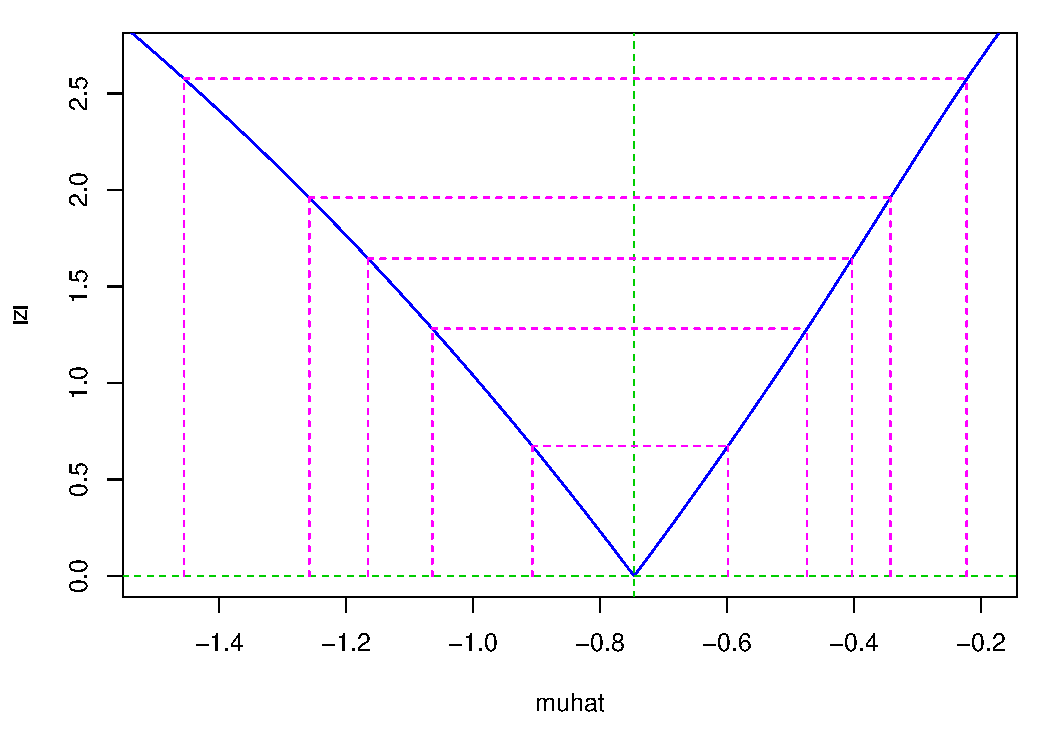
\includegraphics{metaplus-examples-003}
  \caption{Profile plot.}
  \label{fig:profile1}
\end{figure}

The forest plot showing the studies and overall effect can be shown using \texttt{plot(mag.meta)}, and is shown in Figure~\ref{fig:forest1a}. The \textbf{metaplus} package makes extensive use of \textbf{metafor} which allows the parameters for the \texttt{forest} plot in \textbf{metafor} to be used when creating forest plots. As the results for the magnesium studies are actually log odds ratios it is more useful to produce results with units of odds ratios. This can be obtained by annotating the horizontal axis with odds ratios corresponding to the log odds, and requesting an exponential transformation for the coefficients. The plot is shown in Figure~\ref{fig:forest1b}.

\begin{figure}
  \centering
\begin{Schunk}
\begin{Sinput}
> plot(mag.meta)
\end{Sinput}
\end{Schunk}
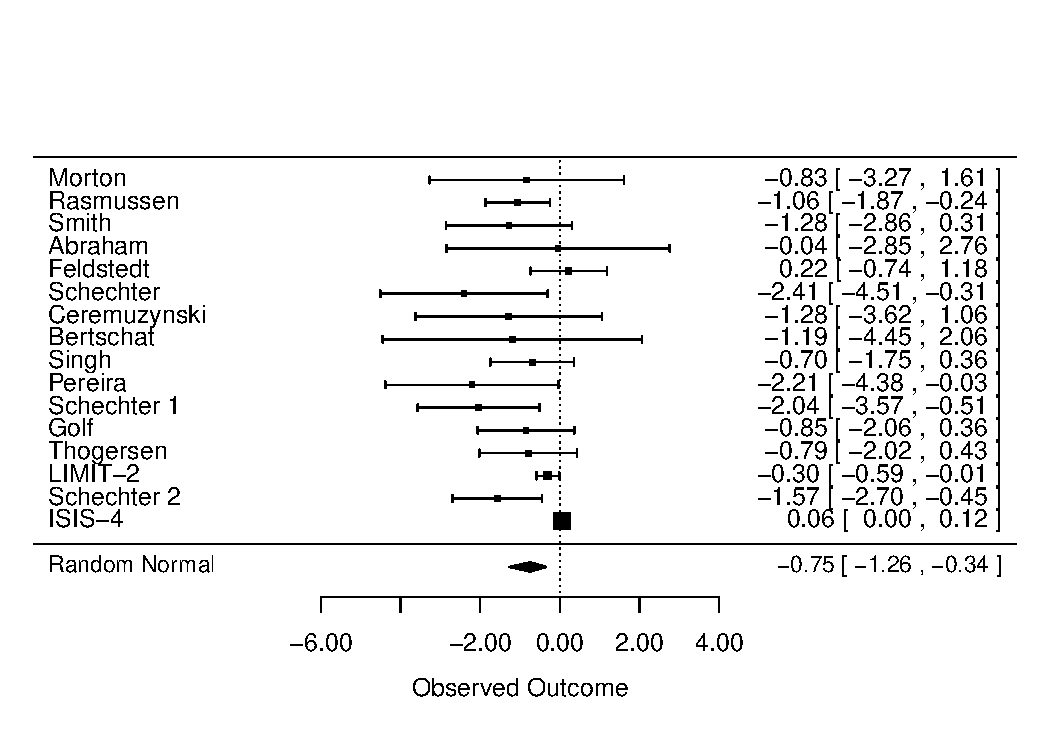
\includegraphics{metaplus-examples-004}
  \caption{Forest plot for Magnesium studies.}
  \label{fig:forest1a}
\end{figure}


\begin{figure}
  \centering
\begin{Schunk}
\begin{Sinput}
> plot(mag.meta,atransf=exp, at=log(c(.01,.1,1,10,100)),xlab="Odds Ratio")
\end{Sinput}
\end{Schunk}
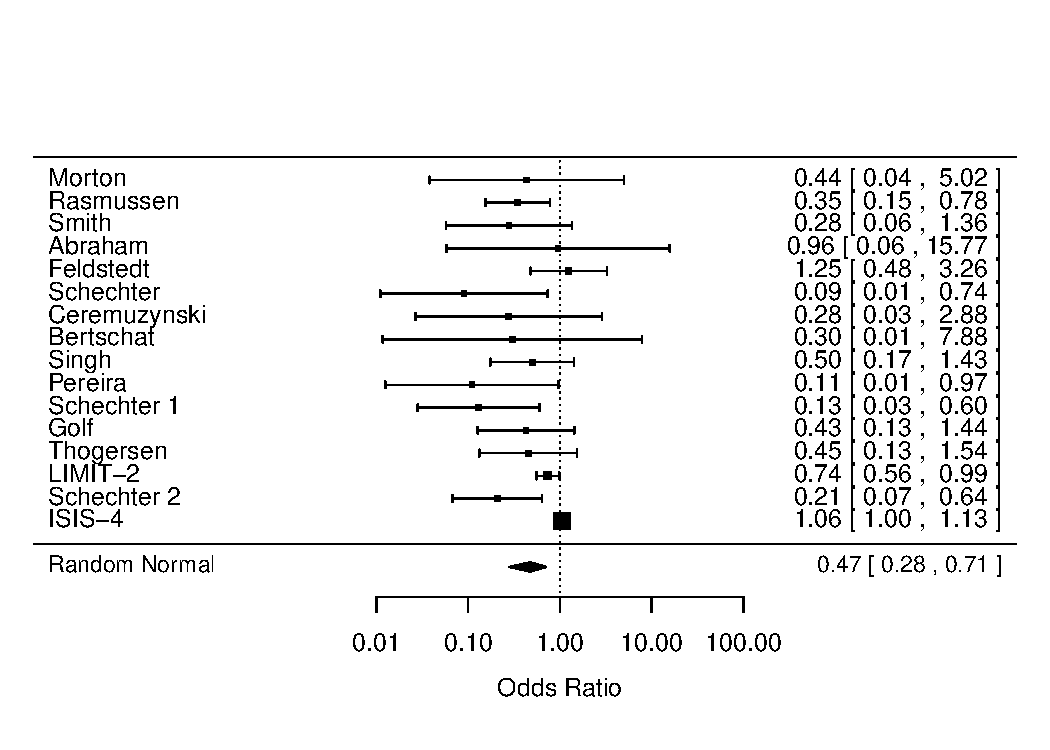
\includegraphics{metaplus-examples-005}
  \caption{Forest plot for Magnesium studies (Odds Ratios).}
  \label{fig:forest1b}
\end{figure}

Repeating the meta-analysis but now allowing for a $t$-distribution for the random effects by adding the \texttt{random="t-dist"}. From the summary the estimate of \texttt{vinv} the inverse degrees of freedom is almost zero, indicating close to infinite degrees of freedom, or a normal distribution.
\begin{Schunk}
\begin{Sinput}
> mag.tdist <- metaplus(mag$yi,mag$sei,slab=mag$study,
+         random="t-dist")
> summary(mag.tdist)
\end{Sinput}
\begin{Soutput}
            Est.      ci.lb      ci.ub   pvalue
muhat -7.463e-01 -1.258e+00 -3.430e-01 0.000501
tau2   2.540e-01                               
vinv   6.051e-11                               

     logLik      AIC      BIC
  -19.68459 45.36918 47.68695
\end{Soutput}
\end{Schunk}

We can confirm this with the \texttt{test.outliers} command, which performs a parametric bootstrap to obtain the null distribution of the likelihood ratio statistic for the test that $v^{-1}=0$, required as the test is on the boundary of the parameter space. Note that this may take some time, of the order of an hour, so it may be better to start with the parameter \texttt{R=99} to limit the number of simulations, with consequently lower accuracy.
\begin{Schunk}
\begin{Sinput}
> summary(test.outliers(mag.tdist))
\end{Sinput}
\begin{Soutput}
Observed LRT statistic 0.0 p value 1
\end{Soutput}
\end{Schunk}

We can repeat using the robust mixture distribution for the random effects. The variance of both the random effect for standard studies (\texttt{tau2}) and for outlier studies (\texttt{tau2out})) are very close indicating that there are no outlier studies and this is confirmed by the outlier test.

\begin{Schunk}
\begin{Sinput}
> mag.mix <- metaplus(mag$yi,mag$sei,slab=mag$study,
+       random="mixture")
> summary(mag.mix)
\end{Sinput}
\begin{Soutput}
                    Est.      ci.lb      ci.ub   pvalue
muhat         -0.7463147 -1.2593989 -0.3427085 0.000777
tau2           0.2539981                               
tau2out        0.2540892                               
Outlier prob.  0.0001904                               

     logLik      AIC      BIC
  -19.68459 47.36918 50.45954
\end{Soutput}
\begin{Sinput}
> summary(test.outliers(mag.mix))
\end{Sinput}
\begin{Soutput}
Observed LRT statistic 0.0 p value 1
\end{Soutput}
\end{Schunk}

\section{CDP choline for Cognitive and Behavioral Disturbances}

This meta-analysis evaluates the effect of CDP choline for cognitive and
behavioral disturbances associated with chronic cerebral disorders in the elderly (cite{Fioravanti2005}). A study (Senin 2003) was previously determined to be an outlier by \citet{Gumedze2011}. We can first fit a standard random effects meta-analysis, as previously.

\begin{Schunk}
\begin{Sinput}
> data(cdp)
> cdp.meta <- metaplus(cdp$yi,cdp$sei,plotci=TRUE,slab=cdp$study)
> summary(cdp.meta)
\end{Sinput}
\begin{Soutput}
         Est.   ci.lb   ci.ub pvalue
muhat 0.38944 0.07269 0.76634 0.0218
tau2  0.14666                       

     logLik      AIC      BIC
  -8.198544 20.39709 21.00226
\end{Soutput}
\end{Schunk}
Note that Senin 2003 does have an unusually high value. We can then fit a robust model using the $t$-distribution.

\begin{Schunk}
\begin{Sinput}
> cdp.tdist <- metaplus(cdp$yi,cdp$sei,plotci=TRUE,slab=cdp$study,
+         random="t-dist")
> summary(cdp.tdist)
\end{Sinput}
\begin{Soutput}
           Est.     ci.lb     ci.ub  pvalue
muhat 1.946e-01 5.296e-02 3.610e-01 0.00899
tau2  4.478e-05                            
vinv  2.024e+00                            

     logLik      AIC      BIC
  -4.057686 14.11537 15.02313
\end{Soutput}
\begin{Sinput}
> summary(test.outliers(cdp.tdist))
\end{Sinput}
\begin{Soutput}
Observed LRT statistic 8.3 p value 0.002
\end{Soutput}
\end{Schunk}
As a rough guide, the improvement in AIC and BIC demonstrate that the model is an improvement, and this is confirmed with the outlier test. We can also perform with the robust mixture.

\begin{Schunk}
\begin{Sinput}
> cdp.mix <- metaplus(cdp$yi,cdp$sei,plotci=TRUE,slab=cdp$study,
+         random="mixture")
> summary(cdp.mix)
\end{Sinput}
\begin{Soutput}
                 Est.   ci.lb   ci.ub  pvalue
muhat         0.19099 0.05586 0.34810 0.00711
tau2          0.00000                        
tau2out       3.15584                        
Outlier prob. 0.12366                        

     logLik      AIC      BIC
  -3.007145 14.01429 15.22463
\end{Soutput}
\begin{Sinput}
> summary(test.outliers(cdp.mix))
\end{Sinput}
\begin{Soutput}
Observed LRT statistic 10.4 p value 0.001
\end{Soutput}
\end{Schunk}
The output from the robust mixture model has an interesting feature. For standard studies the estimated random effects variance is zero, indicating that only the outlier studies are contributing to the heterogeneity. The posterior probability of each study being an outlier can be obtained as:
\begin{Schunk}
\begin{Sinput}
> cdp.mix.outlier.probs <- outlier.probs(cdp.mix)
\end{Sinput}
\end{Schunk}
and plotted as in Figure~\ref{fig:outliers2}. This shows clearly that Senin 2003 does have a posterior probability of nearly 1.0 of being an outlier. The other studies have some posterior probability of being outliers, as there is an overlap between the distribution of the standard and outlier studies.

\begin{figure}
  \centering
\begin{Schunk}
\begin{Sinput}
> plot(cdp.mix.outlier.probs)
\end{Sinput}
\end{Schunk}
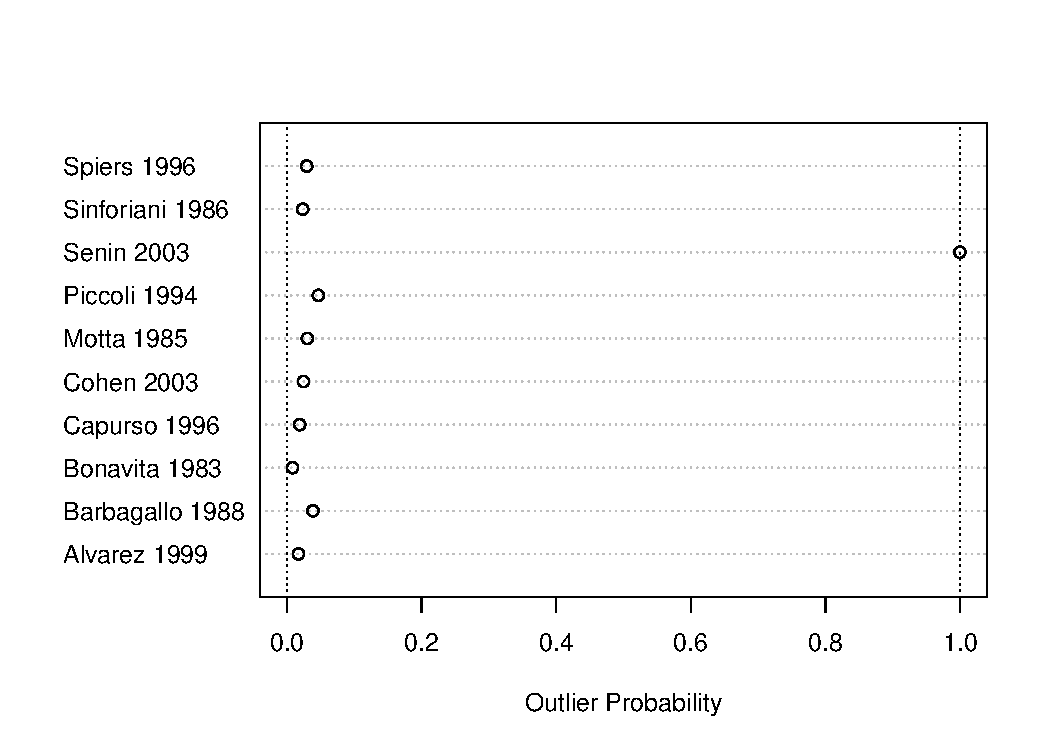
\includegraphics{metaplus-examples-013}
  \caption{Outlier probabilities for CDP studies}
  \label{fig:outliers2}
\end{figure}

Lastly, we can now produce a forest plot with the results of all three models, using the \texttt{extrameta} parameter to add the robust models, and these are shown in Figure~\ref{fig:forest2}. The effect of the robust models is to down-weight the Senin 2003 study, which has the consequence of both reducing the overall effect estimate and the standard error.

\begin{figure}
  \centering
\begin{Schunk}
\begin{Sinput}
> plot(cdp.meta,extrameta=list(cdp.tdist,cdp.mix))
\end{Sinput}
\end{Schunk}
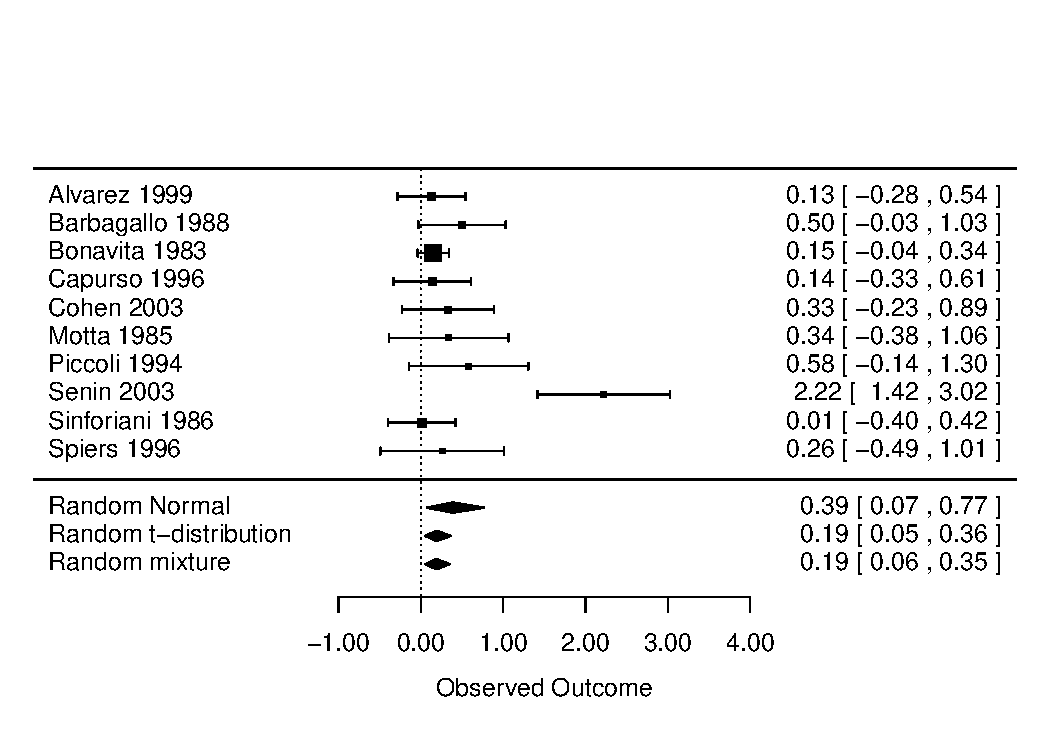
\includegraphics{metaplus-examples-014}
  \caption{Forest plot for CDP Studies.}
  \label{fig:forest2}
\end{figure}

\subsection{Exercise for Depression}

This example is a meta-analysis of trials of exercise in the management of depression \cite{Lawlor2001}. \citep{Higgins2004} used the data as in example of meta-regression, and a number of covariates, which will be limited here to a single covariate duration of trial. First performing the meta-analysis using standard normal random effects and the robust mixture model. 

\begin{Schunk}
\begin{Sinput}
> data(exercise)
> exercise.meta <- metaplus(exercise$smd,sqrt(exercise$varsmd),
+       mods=exercise[,c("duration"),drop=FALSE],slab=exercise$study)
> summary(exercise.meta)
\end{Sinput}
\begin{Soutput}
            Est.   ci.lb   ci.ub   pvalue
muhat    -2.8994 -4.3006 -1.5222 0.000884
tau2      0.1171                         
duration  0.2078  0.0584  0.3632 0.011570

     logLik      AIC      BIC
  -8.133435 22.26687 23.17462
\end{Soutput}
\begin{Sinput}
> exercise.mix <- metaplus(exercise$smd,sqrt(exercise$varsmd),
+       mods=exercise[,c("duration"),drop=FALSE],
+       slab=exercise$study,random="mixture")
> summary(exercise.mix)
\end{Sinput}
\begin{Soutput}
                  Est.    ci.lb    ci.ub   pvalue
muhat         -2.88472 -4.11371 -1.48419 0.000649
tau2           0.00000                           
tau2out        0.59398                           
Outlier prob.  0.25169                           
duration       0.21086  0.07429  0.34608 0.007052

    logLik      AIC     BIC
  -7.69139 25.38278 26.8957
\end{Soutput}
\begin{Sinput}
> exercise.test.outliers <- test.outliers(exercise.mix)
> summary(exercise.test.outliers)
\end{Sinput}
\begin{Soutput}
Observed LRT statistic 0.9 p value 0.077
\end{Soutput}
\begin{Sinput}
> exercise.outlier.probs <- outlier.probs(exercise.mix)
\end{Sinput}
\end{Schunk}

The test for outliers was close to significant (p=0.077), however a conservative approach seems appropriate, by using the robust model where the presence of outliers is not conclusive but there is a reasonable amount of evidence that there are outliers, as in this case. Note also that the p value is different from that obtained in the Beath (2014) paper, due to the use of a parametric bootstrap, which uses randomly generated data. Running parametric bootstrap with a large number of simulations showed that the p value was in fact near 0.04. From Figure~\ref{fig:outprobs3} the study by Reuter is an obvious outlier with a posterior probability greater than 0.9. This study is a dissertation and was not published in a peer-reviewed journal, and was not included in a later meta-analysis by \citet{Krogh2011}.


\begin{figure}
  \centering
\begin{Schunk}
\begin{Sinput}
> plot(exercise.outlier.probs)
\end{Sinput}
\end{Schunk}
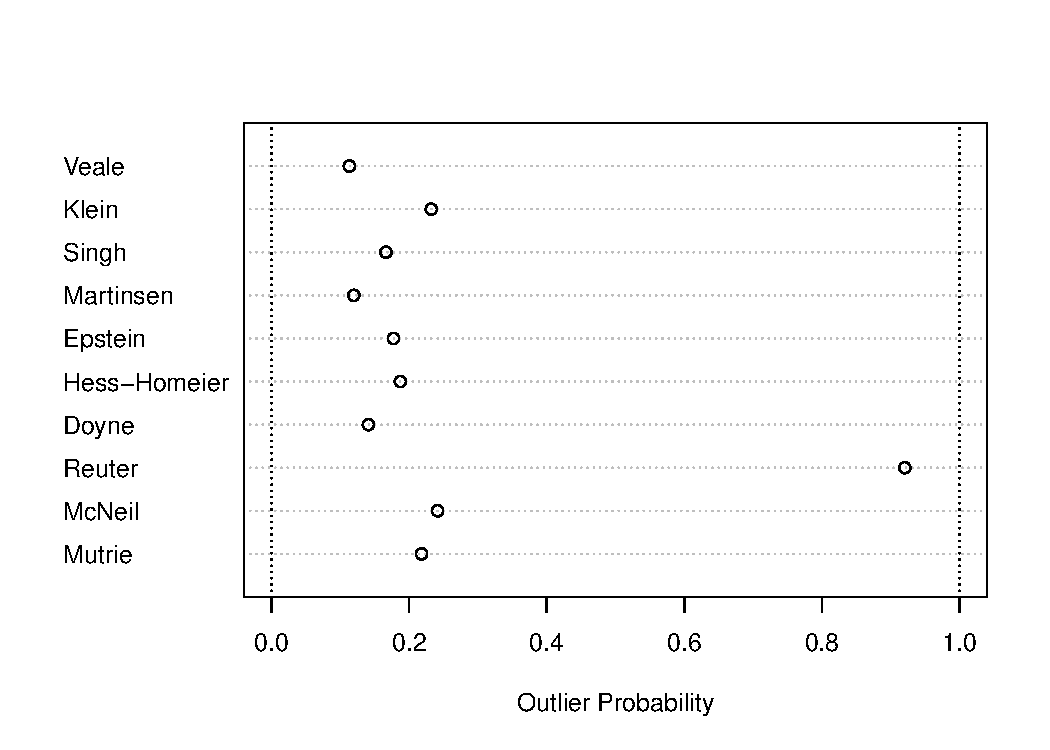
\includegraphics{metaplus-examples-016}
  \caption{Outcome Probabilities for Depression versus Exercise.}
  \label{fig:outprobs3}
\end{figure}

To calculate the effect at each of Weeks 4, 8 and 12 it is easiest to center the data at those times and fit a meta-regression for each. The intercept for each meta-regression will then be the prediction at that time. We also fit a model without including the covariate for study duration. The forest plot is shown in Figure~\ref{fig:forest3}. This shows that the effect of exercise decreases rapidly the longer the trial, possibly indicating a placebo effect that rapidly wears off. It would also be possible to plot the results from the standard random effects models as well.

\begin{Schunk}
\begin{Sinput}
> exercise$duration4 <- exercise$duration-4
> exercise$duration8 <- exercise$duration-8
> exercise$duration12 <- exercise$duration-12
> exercise.nodurn <- metaplus(exercise$smd,sqrt(exercise$varsmd),
+     label="Random Mixture (No Duration)",slab=exercise$study,
+     random="mixture")
> exercise.wk4 <- metaplus(exercise$smd,sqrt(exercise$varsmd),
+     mods=exercise[,c("duration4"),drop=FALSE],plotci=TRUE,
+     label="Random Mixture (Week 4)",slab=exercise$study,
+     random="mixture")
> exercise.wk8 <- metaplus(exercise$smd,sqrt(exercise$varsmd),
+     mods=exercise[,c("duration8"),drop=FALSE],
+     label="Random Mixture (Week 8)",slab=exercise$study,
+     random="mixture")
> exercise.wk12 <- metaplus(exercise$smd,sqrt(exercise$varsmd),
+     mods=exercise[,c("duration12"),drop=FALSE],
+     label="Random Mixture (Week 12)",slab=exercise$study,
+     random="mixture")
\end{Sinput}
\end{Schunk}


\begin{figure}
  \centering
\begin{Schunk}
\begin{Sinput}
> plot(exercise.nodurn,extrameta=list(exercise.wk4,exercise.wk8,
+       exercise.wk12))
\end{Sinput}
\end{Schunk}
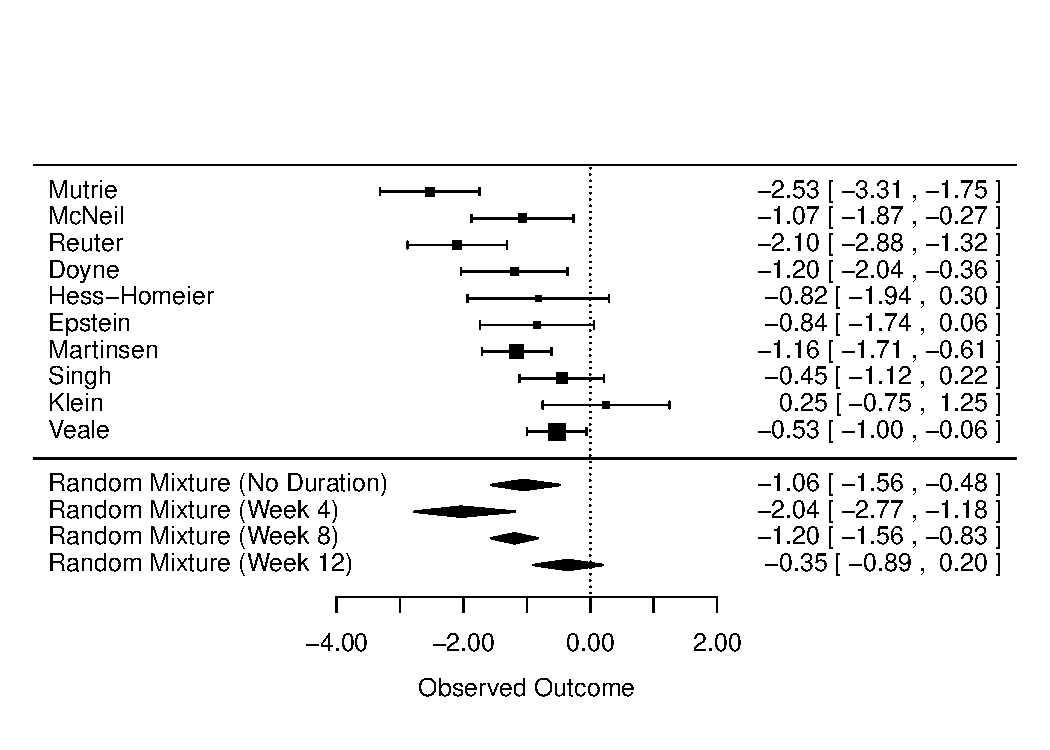
\includegraphics{metaplus-examples-018}
  \caption{Forest plot for Exercise versus Depression studies.}
  \label{fig:forest3}
\end{figure}

\bibliography{metaplus-examples}

\end{document}
